\chapter{3D Phase Tracking Monte Carlo Algorithm}\label{sec:phase}

\section{Introduction}\label{sec:besintro}

Bessel beams have been the subject of intense research since their discovery in 1987~\cite{durnin1987diffraction,durnin1987exact}. Durnin noticed that the blah blah.
Bessel beams have since been used for blah blah
They are really good and like are better than Gaussian beams allegedly.

This chapter examines how Bessel beams compare to other beam in a scattering medium. 
We investigate if the Bessel beams self-healing property has any effect in a turbid medium.
We examine Bessel beams and the other beams by creating a novel~\gls{mcrt} algorithm that allows the tracking of a photon as it propagates through a medium. 
The main focus of this chapter, is validation of our new novel technique, followed by using the new algorithm ($\varphi MC$) to compare Gaussian and Bessel beams, to see which one preforms better in a turbid medium. 
This chapter also extends out novel algorithm to other complex, diffraction less beams


motivation => better imaging of chick embryos etc


\section{Theory}\label{sec:bestheory}

The \gls{mcrt} algorithm as described in~\cref{sec:mcrt}, must be adjusted so that wave phenomena such as interference and diffraction can be modelled. 
Modelling these wave behaviours allows us to model complex beams, where these phenomena are required to form the beam, e.g Bessel beams. 
As \gls{mcrt} is a ballistic simulation of photon packets, meaning that the \gls{mcrt} simulation presented thus far in this thesis only modelled the ballistic behaviour of photons. 
However for the work presented in this chapter, wave like behaviours is crucial to modelling the various experiments and phenomena.

In order to convert a ballistic simulation of photon packets into a ballistic/wave-like simulation, the complex phase of each photon packet is tracked.
This is achieved, by simply tracking the complex phase of the photon as it propagates through a medium.
~\Cref{eqn:phase} shows how the phase is calculated.

\begin{equation}
    \varphi = cos\left(\frac{2 \pi l}{\lambda}\right) + i\ sin\left(\frac{2 \pi l}{\lambda}\right)
    \label{eqn:phase}
\end{equation}

Where $\varphi~[-]$ is the phase of a photon packet, $l\ [m]$ is the distance the photons has travelled, and $\lambda~[m]$ is the wavelength of the photon.
Now we can calculate the phase of a photon at a position $\hat{p_o}$, if we know the distance it has travelled, and its original phase. 
To be able model the wave-like behaviour of photons, we let the photons packets interfere with one another in a volume or area element. 
We do not model the interference at just the points where photons packets cross one another as due to the ballistic nature of the \gls{mcrt} simulation, this does not occur with enough frequency in order to give a good signal to noise ratio. 
The interference takes place in a volume element $dV$ or area element $dA$ instead.
To calculate the interference from the phase, the phase if summed in each volume or area element and the absolute value taken, and then squared.~\Cref{eqn:intense} shows the equation for interference for a volume element $dV$.

\begin{equation}
I(\xi)=\left| \sum\limits_{\xi}cos\left(\frac{2\pi d}{\lambda}\right) + i \sum\limits_{\xi}sin\left(\frac{2\pi d}{\lambda}\right)\right|^2,\ \ \ \xi=(x,y,z)
\label{eqn:intense}
\end{equation}

\noindent Where:

\indent $l$ is the total distance travelled by a photon [$m$];

\indent $\lambda$ is the wavelength of the photon [$m$];

\indent $I$ is the intensity at the $\xi^{th}$ cell [dunno];

\indent and $\xi$ is the $x^{th}$, $y^{th}$, $z^{th}$ cell, volume $dV$.

\medskip

As the \gls{mcrt} simulation is now a quasi ballistic/wave simulation of photon behaviour, we compare our simulations to theoretical and experimental data to prove this model is accurate. However before we validate our model we first introduce one further principle that is required for our model to work.

\subsection{Huygens-Fresnel Principle}

The Huygens-Fresnel principle is a method that is used to help mode the propagation of waves in the far-field limit and the near-field limit. 

The Huygens principle: Every point point on a wavefront acts as a source of spherical wavelets, and that the sum of all the wavelets forms the wavefront. 
The principle is illustrated in~\cref{fig:huygensillis}. 
Fresnel later came along and fixed, then kirchoff double fixed it real good, with math and stuff.


allows us to calculate complex amplitude at a given point. 
inclination factor no backward waves.
used in diffraction theory -> kirchoffs

fresnel and fraunhoefer diffraction -> validation of algorithm
fresnel close
fraunhoefer far away

\begin{figure}[!ht]
    \centering
    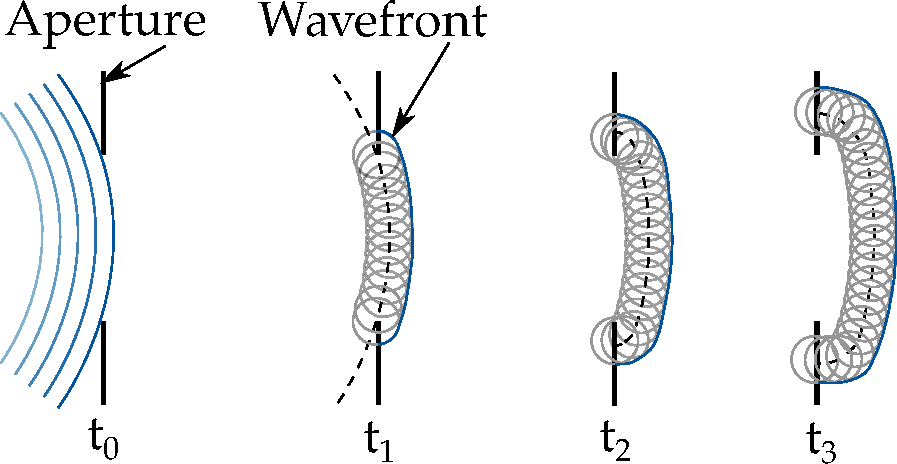
\includegraphics[width=0.95\textwidth]{huygens.pdf}
    \caption{Illustration of the Huygens-Fresnel principle. At $t_0$ a wave is incident on an aperture. Times $t_1,\ t_2,\ \text{and}\ t_3$ show the evolution of the wavefront using the Huygens-Fresnel principle.}
    \label{fig:huygensillis}
\end{figure}

\subsection{Validation of Phase Tracking Algorithm}

The first test of our phase tracking algorithm, is to compare our simulation to a double slit experiment.
The double slit experiment, is a simple experiment where monochromatic plane wave of light is incidence on two slits, and the interference pattern is observed on a screen a distance $d$ away from the slits.

In this experiment blah bla ***

\begin{equation}
    I(\theta) \propto cos^2\left(\frac{\pi d\ sin \theta}{\lambda}\right)sinc^2\left(\frac{\pi b\ sin\theta}{\lambda}\right)
\end{equation}
Where the $sinc$ function is defined as $\tfrac{sin(x)}{x}$, for $x\ \neq 0$, b is the slit width, d is the slit separation and $\theta$ is the angular spacing of the fringes.

\section{Bessel Beams}


\begin{figure}[!ht]
    \centering
    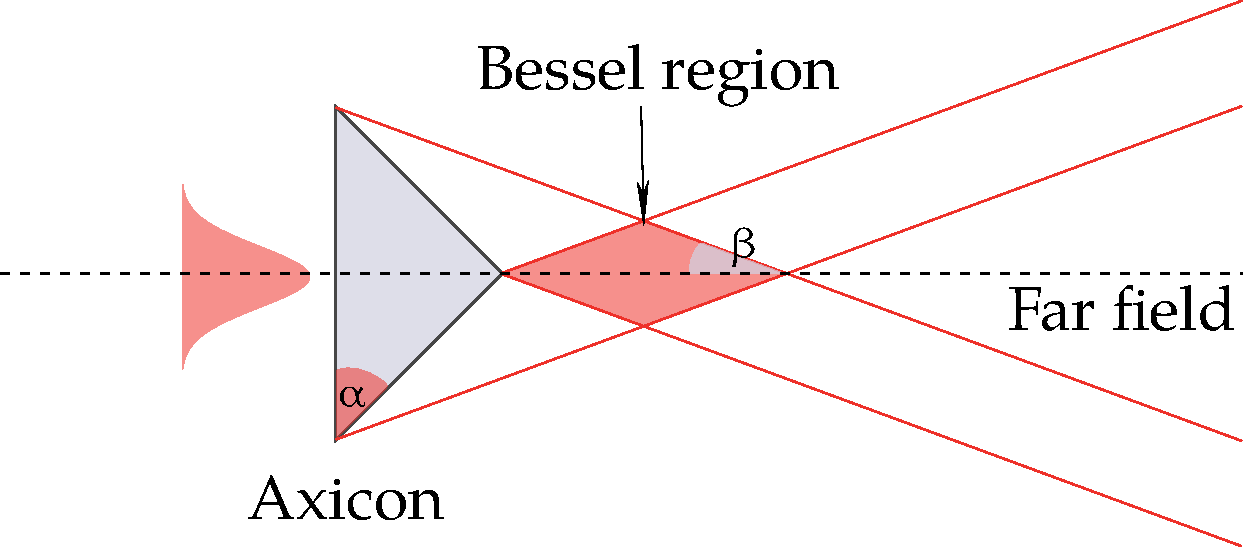
\includegraphics[width=0.95\textwidth]{bessel.pdf}
    \caption{Geometry of a Bessel beam, generated by an axicon lens. $\beta$ is the angle with the optical axis, and the angle of the conical waves. $\alpha$ is the axicon angle.}
    \label{fig:besselgeo}
\end{figure}

From the scalar description of the electric component of the beam, we get:

\begin{equation}
    E(r,z)=E_0\sqrt{\frac{2\pi k z w_0sin(\beta)}{z_{max}}}\ \text{exp}^{\left(-\frac{z^2}{z_{max}^2}-\frac{i\pi}{4}\right)}\ J_0\left(krsin(\beta)\right)\ \text{exp}^{\left(ikzcos(\beta)\right)}
    \label{eqn:besselEfield}
\end{equation}

\noindent Where:

    \indent k is the wavevector, $k=\tfrac{2\pi}{\lambda}$ [$m$];

    \indent z is the distance from the axicon tip [$m$]; 

    \indent $\beta$ is the angle the wavefront propagates at (see~\cref{fig:besselgeo}) [$rad$]; 

    \indent $w_0$ is the $\tfrac{1}{e^2}$ width of the input Gaussian beam [$m$]; 

    \indent $J_0$ is the Bessel function of the first order; 

    \indent r is radial distance from the optical axis [$m$]. 

\medskip


~\Cref{eqn:besselEfield} gives the electric field for a Bessel beam. The intensity can be calculated using:

\begin{equation}
    I(r,z)=\frac{c\epsilon_0\left|E_0\right|^2}{2}
    \label{eqn:besselintsub}
\end{equation}

Using the definition total power transmitted by a beam as:

\begin{equation}
    P=\frac{\pi I_0w_0^2}{2}
    \label{eqn:pwrdef}
\end{equation}

Where $I_0$ is defined as on axis intensity of the incident Gaussian beam.

\begin{equation}
    I_0=\frac{c\epsilon_0E_0^2}{2}
    \label{eqn:intdef}
\end{equation}

Substituting~\cref{eqn:besselEfield,eqn:intdef,eqn:pwrdef} into~\cref{eqn:besselintsub} yields:

\begin{equation}
    I(r,z)=\frac{4k_rP}{w_0}\frac{z}{z_{max}}J_0^2\left(k_r\ r\right)\text{exp}^{\left(-\frac{2z^2}{z^2_{max}}\right)}
    \label{eqn:besselInt}
\end{equation}


\noindent Where:

    \indent $k_r$ is the radial wavevector, $k_r=k sin(\beta)$;

    \indent P is the power of the incident Gaussian beam.

    \medskip

To check out method accurately models Bessel beams, we compare out beam to theoretical expressions and experimental data.

To compare against a theoretical Bessel beam, a Bessel beam is modelled in the MCRT phase simulation, and propagated through air past the ``Bessel region''. 
A slice of the intensity is then plotted against what the theory predicts the Bessel beam should look like. 
A check of how the Bessel beam propagates in the far field is also preformed.


~\Cref{eqn:besselInt} gives the profile of a theoretical Bessel beam at a depth $z_{max}$, this is plotted against the simulation when $\tfrac{4k_rPz}{w_0z_{max}}e^{-2\left(\tfrac{z}{z_{max}}\right)^2}=1$, with the simulation normalised to a maximum of 1 as well. ~\Cref{fig:besselCompare} shows this comparison.


\begin{figure}[!ht]
    \centering
    % \includegraphics[]{}
    \caption{Comparison of theoretical and MCRT simulation of a Bessel beams, with intensity normalised.}
    \label{fig:besselCompare}
\end{figure}

To ensure our algorithm works in turbid media, we carried out an experiment where a Bessel beam was propagated through a medium of varying turbidity.
A laser, wavelength $488~nm$, with a Gaussian profile is shone on an axicon lens, with angle $5~^{\circ}$.
The laser beam had a $\tfrac{1}{e^2}$ spot size of $2~mm$. 
The Bessel beam was allowed to propagate through the air for $10~cm$ before entering a cuvette of side $2~mm$.
The cuvette was filled with $500~\mu L$ of water, and various volumes of a scattering agent added.
The scattering agent used is intralipid $20~\%$, which is diluted as shown in~\cref{tab:intra}.
Images of the Bessel as it emerges from the cuvette are taken for comparison with out algorithm.
~\Cref{fig:expsetup} shows the experimental setup.

\begin{figure}[ht!]
    \centering
    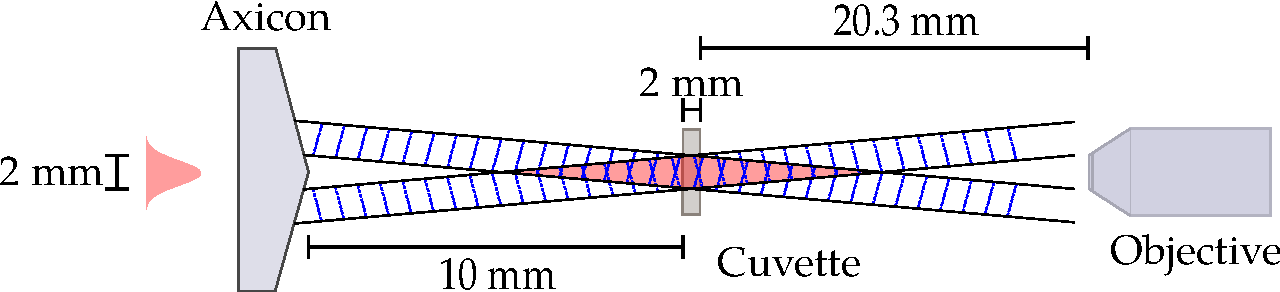
\includegraphics[width=0.95\textwidth]{bessel-exp-setup.pdf}
    \caption{Experimental setup for propagating a Bessel beam through a cuvette filled with varying concentrations of Intralipid 20\%. Bessel beam is imaged by an 20x objective lens and a Grasshopper 3 camera.}
    \label{fig:expsetup}
\end{figure}

\begin{table}[!ht]
    \centering
    \begin{tabular}{ccc}
    \hline
    \multicolumn{3}{c}{Volume/$\mu L$}                                               \\ \hline
    Intralipid              & $H_2O$                   & Intralipid concentration/\% \\ \hline
    \multicolumn{1}{c|}{0}  & \multicolumn{1}{c|}{500} & 0                           \\
    \multicolumn{1}{c|}{2}  & \multicolumn{1}{c|}{500} & 0.39841                     \\
    \multicolumn{1}{c|}{4}  & \multicolumn{1}{c|}{500} & 0.79365                     \\
    \multicolumn{1}{c|}{6}  & \multicolumn{1}{c|}{500} & 1.18577                     \\
    \multicolumn{1}{c|}{8}  & \multicolumn{1}{c|}{500} & 1.57480                     \\
    \multicolumn{1}{c|}{10} & \multicolumn{1}{c|}{500} & 1.96078                     \\
    \multicolumn{1}{c|}{12} & \multicolumn{1}{c|}{500} & 2.34375                     \\ \hline
    \end{tabular}
    \caption{Intralipid solutions used for experiment.}
    \label{tab:intra}
\end{table}


To model the experimental setup we simplify the setup considerably.
The simulation setup models just the phase delay of the axicon on the laser beam and the beams propagation through the cuvette onto an image plane. 

% \begin{figure}
% \centering
% 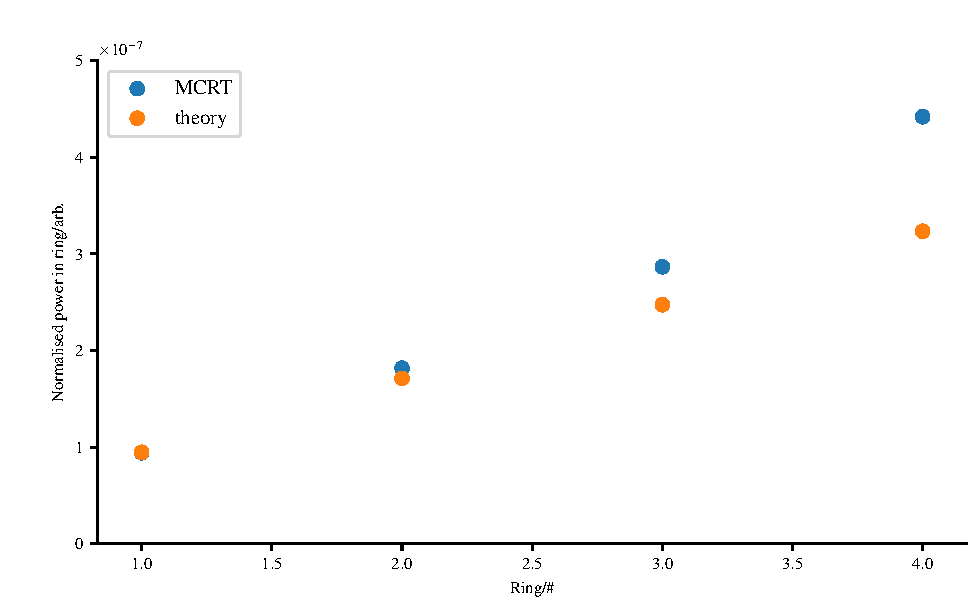
\includegraphics[scale=0.65]{pwr-rings.pdf}
% \caption{Bessel beam power in each ring.}
% \label{fig:pwrring}
% \end{figure}

\begin{figure}
\centering
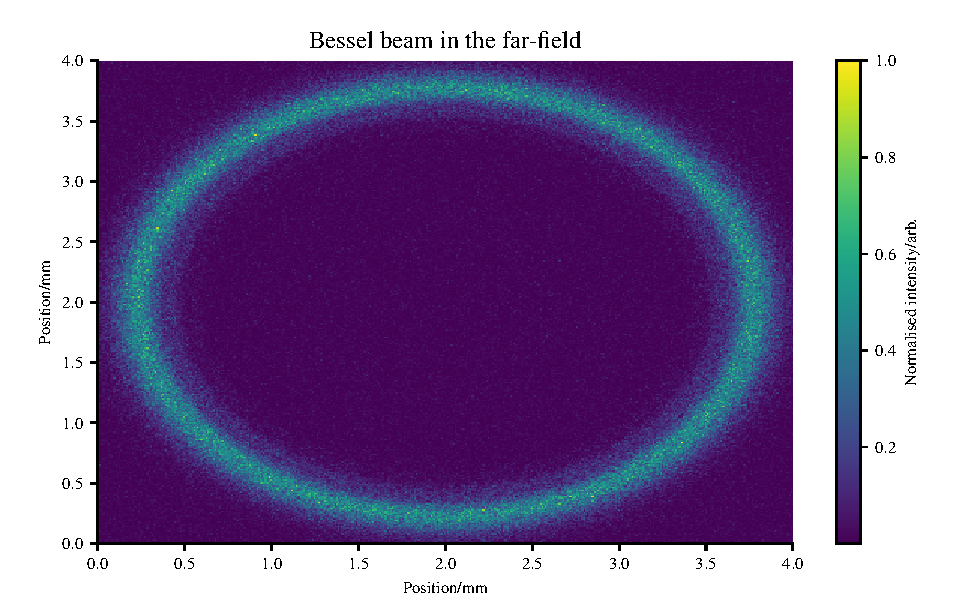
\includegraphics[scale=0.75]{far-field.pdf}
\caption{Bessel beam in the far field.}
\label{fig:farfield}
\end{figure}
\section{Gaussian Beams}

implementation of lenss -> plano-convex and aspheric
emphasis no coding of focal distance
spherical aberrations 
curvature of phase change

need to find factor root 2

\section{Other Beams}

Our technique outlined in the preceding sections, can also be applied to arbitrary non-diffracting or complex beams. The only requirements for our algorithm to be able to model a complex beam, is that there is some phase delay that can be modelled analytically\footnote{It may be possible to model phase delays that are not analytical expressions. Simulating spatial light modulators may also be possible with our algorithm.}.

The first example of using our algorithm to model complex beams is to model a Laguerre-Gauss beam. A Laguerre-Gauss beam can be created by introducing a helical phase delay to a plane wave blah blah. ***put theory here + phase and interference patterns for all beams

Another example of our algorithms flexibility is that it can also model Hermite-Gauss beams, higher order Bessel beams and airy beams

\section{Comparison}

\section{Discussion}

talk about comparison of beams. methods validity -> downside and upsides

a~\cite{mignon2016fractional}
\section{Conclusion}

conclude shit


sources
cizmar thesis
born: principles of optics
hecht: optics
mignon
prahl
fresnel/fraunhoefer paper
thorlabs
sacsha thesis
kishans papers
various axicon papers
aspheric papers
phase screen model
beam steering paper
paper that hates on mcrt
E-field mcrt